\documentclass[]{article}
\usepackage{graphicx}
\usepackage{hyperref}
\usepackage{amsmath}
\usepackage{caption}
\usepackage{subcaption}
\usepackage{ngerman}
\usepackage[utf8]{inputenc}
\usepackage{float}

%opening
\title{Hochauflösende $\gamma$ Spektroskopie}
\author{Gunther T\"urk, Jonas Lehnen}

\begin{document}

\maketitle
\begin{abstract}
In diesem Experiment wollen wir verstehen wie der $\gamma$ Zerfall gemessen wird um die genaue Energie des Photons zu bestimmen. Nach dem ein Elektron gefangen oder ein $\beta$ Zerfall statt fand, ist der Atomkern angeregt. Die Abregung des Kerns erfolgt über eben dieses Photon, welches ein Germanium Detektor messen kann. In diesem Zuge werden wir besprechen in wie weit Elektronik und Hintergrundstrahlung dieses Experiment beeinflussen.
\end{abstract}

\tableofcontents


\newpage
\section{Theorie}
\subsection{Radioaktive Strahlung}
Grundsätzlich existieren drei Arten des radioaktiven Zerfalls. Beginnend mit dem $\alpha$ Zerfall, bei dem ein ${He}\ ^{2+}$ Teilchen aus einem größeren Atomkern emittiert wird. Die genauen Zerfallskanäle sind in Tabelle \ref{tab:zerfall} dargestellt. $\alpha$ Strahlung selbst ist leicht abgeschirmt, so besteht bereits nach $10cm$ Luftweg keine Belastung für Menschen. Probleme entstehen erst bei Alphastrahlern im Körper, da dann die gesamte Energie deponiert wird und unter anderem Krebs auslösen kann.

\renewcommand{\arraystretch}{2}
\begin{table}[H]
\centering
\begin{tabular}{c||c}
Zerfallsart & Formel   \\ \hline
$\alpha$ & $_Z^A X \rightarrow\ _2^4\alpha + _{Z-2}^{A-4} Y$ \\ \hline
$\beta^+$ &   $_Z^A X \rightarrow\  _{Z-1}^{A}Y + e^+ + \nu_e$ \\ \hline
$\beta^-$ &   $_Z^A X \rightarrow\  _{Z+1}^{A}Y + e^- +  \bar{\nu}_e$ \\ \hline
$\gamma$ &  $_Z^A X^* \rightarrow\ _Z^A X + \gamma$  \\ \hline
$EC$ &   $_Z^A X  + e^- \rightarrow\ _{Z-1}^{A}Y + \nu_e $
\end{tabular}
\caption{Darstellung aller möglichen radiokativen Zerfälle. Die Kernendprodukte können sich, bis auf beim $\gamma$ Zerfall, noch in einem angeregten Zustand befinden. Dies wird durch $X^*\ bzw.\ Y^*$ dargestellt.  }
\label{tab:zerfall}
\end{table}
\renewcommand{\arraystretch}{1}

Wie in jedem Zerfall gilt auch für die $\beta$ Zerfälle, dass die Masse des ursprünglichen Kerns größer ist als die der Zerfallsprodukte. Dies liegt an der Energieerhaltung, da zusätzliche kinetische Energie entsteht um das Zerfallsteilchen fort zubewegen. Hier unterscheidet man je nach Ladung von Elektron oder Positron zwischen negativen um positiven $\beta$ Zerfall. Damit auch die Flavourerhaltung der Leptonen berücksichtigt wird, entstehen hierbei zusätzliche Neutrinos. Im Kern selbst zerfällt dabei ein Neutron bzw. Proton zu genau dem anderen Kernteilchen. Der Zerfall eines freien Protons ist theoretisch möglich jedoch wird die Halbwertszeit auf $10^{35}$ Jahre geschätzt. Unser Universum ist bisher erst ca. $10^{10}$ Jahre alt. Es ist also sehr unwahrscheinlich einen solchen Nachweis in einem Menschenleben erbringen zu können.

Alle genannten Strahlungsarten können nun in einem angeregten Kernzustand enden. An dieser Stelle setzt nun der $\gamma$ Zerfall ein. Diese angeregten Zustände sind durch Kernspin und Parität charakterisiert. Dieser Zerfall entspricht einer Umstrukturierung des Kernaufbaus und die dabei gewonnene Energie hat zwei Möglichkeiten umgesetzt zu werden. Entweder als Photon des $\gamma$ Zerfalls oder auch direkt an ein Elektron, welches dann das Atom verlassen kann, sofern die Bindungsenergie aufgebracht werden konnte. Dieser Prozess wird Innere Umwandlung genannt und kann nur mit Elektronen einer s-Schale stattfinden, da nur diese eine Aufenthaltswahrscheinlichkeit im Kern besitzen.

\begin{figure}[H]
\centering
\begin{subfigure}[b]{.48\textwidth}
\centering
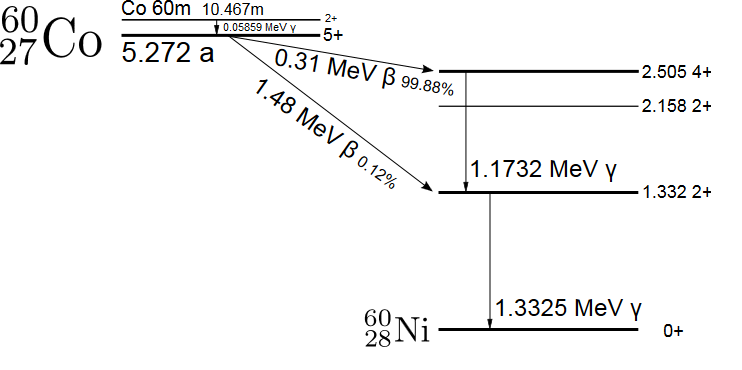
\includegraphics[width=1\textwidth]{Plots/Cobalt1.png}
\caption{Schema der Energieniveaus und Zerfallsübergänge. Vor dem eigentlichen $\gamma$ Zerfalls findet ein $\beta^-$ Zerfall statt. Am rechten Rand sind Kernspin und Parität vermerkt. Die Halbwertszeit ist mit mit 5.272 Jahren ebenfalls dargestellt.}
\end{subfigure}
\begin{subfigure}[b]{.48\textwidth}
\centering
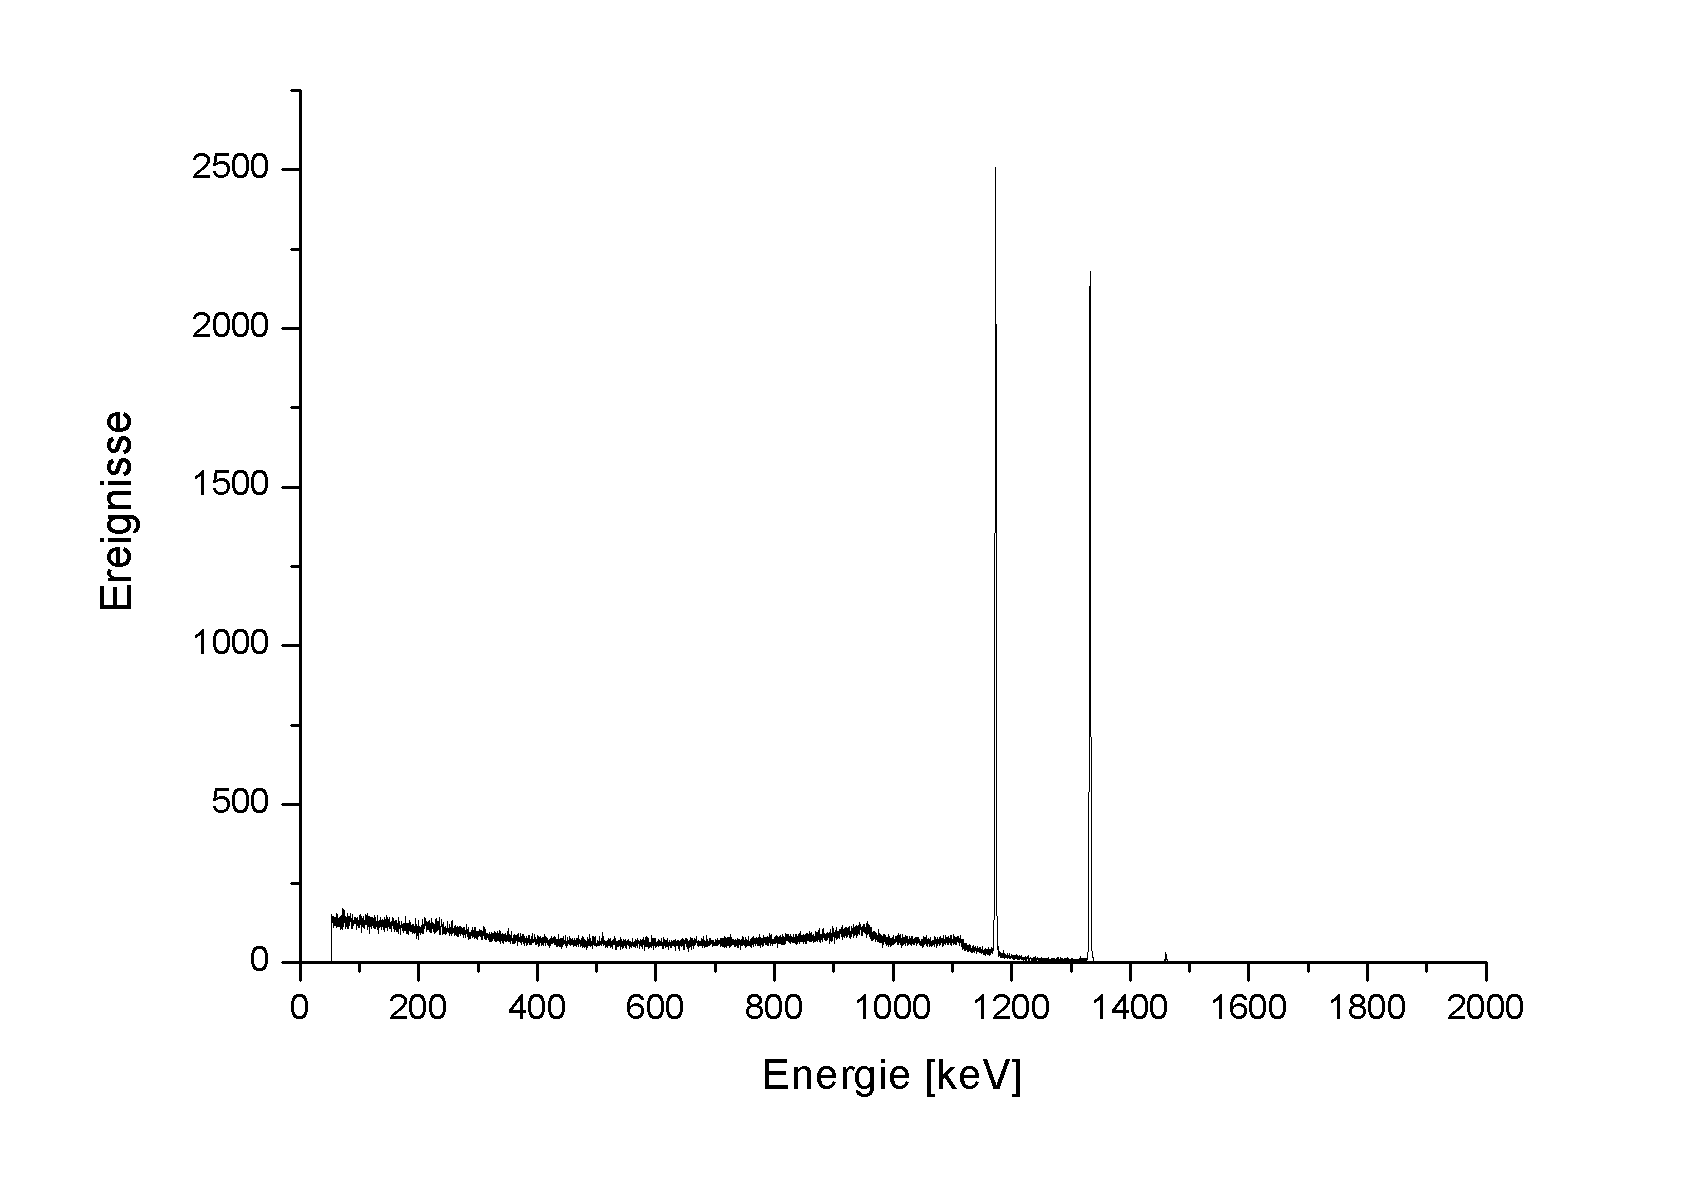
\includegraphics[width=1.1\textwidth]{Plots/Cobalt2.png}
\caption{Spektrum des $\gamma$ Zerfalls. Beide Peaks entsprechen den im $^{60}Ni$ angegebenen Energien des Übergangs. }
\end{subfigure}
\caption{Darstellungen des $\gamma$ Zerfalls vom $^{60}Co$. \cite{cobalt}}
\end{figure}

Zusätzlich existiert noch der Gegensatz zum $\beta$ Zerfall. Beim Electron Capture EC wird ein Elektron eingefangen statt ausgesendet. Durch die Änderung des Kerns befindet sich jetzt das gesamte Atom in einem angeregten Zustand, statt der Kern. Am wahrscheinlichsten ist, dass ein $e^-$ aus der K-Schale gefangen wird. Dabei entsteht ein freier Platz auf einem niedrigen Niveau, welcher dann von oben wieder nach besetzt wird. Dabei entsteht nun Röntgenstrahlung, statt $\gamma$ Strahlung. Der Unterschied zwischen besteht also darin, ob das Photon im Kern ($\gamma$) oder aus der Schale (Röntgen) stammt.

%%% Zur Vollständigkeit wird noch das Zerfallsgesetz angegeben?
%%% Aktivität dazu vll?


\subsection{Photonische Wechselwirkung mit Materie}
\subsection{Detektion von Strahlung}
%%% schintillator kurz, germanium halbleiter, pmt
%%% Beschreibung vom Spektrum, erwartete grafik



\newpage
\section{Experiment}
\subsection{Setup}
%%% Signal verarbietung?


\newpage
\section{Anhang}


\newpage
\begin{thebibliography}{}

\bibitem{protonzerfall} \begin{verbatim}
https://de.wikipedia.org/wiki/Protonenzerfall
\end{verbatim}

\bibitem{cobalt} \begin{verbatim}
https://en.wikipedia.org/wiki/Cobalt-60
\end{verbatim}

\end{thebibliography}
\end{document}

